\documentclass{article}

\def\npart{III}
\def\nyear{2018}
\def\nterm{Michaelmas}
\def\nlecturer{Dr. P. Varj\'{u}}
\def\ncourse{Topics in Ergodic Theory}
\def\draft{Ongoing course, rough}

\usepackage{imakeidx}
\usepackage{marginnote}

\ifx \nauthor\undefined
  \def\nauthor{Bhavik Mehta}
\else
\fi

\author{Based on lectures by \nlecturer \\\small Notes taken by \nauthor}
\date{\nterm\ \nyear}
\title{Part \npart\ -- \ncourse}

\usepackage[utf8]{inputenc}
\usepackage{amsmath}
\usepackage{amsthm}
\usepackage{amssymb}
\usepackage{enumerate}
\usepackage{mathtools}
\usepackage{graphicx}
\usepackage[dvipsnames]{xcolor}
\usepackage{tikz}
\usepackage{wrapfig}
\usepackage{centernot}
\usepackage{float}
\usepackage{braket}
\usepackage[hypcap=true]{caption}
\usepackage{enumitem}
\usepackage[colorlinks=true, linkcolor=mblue]{hyperref}
\usepackage[nameinlink,noabbrev]{cleveref}
\usepackage{nameref}
\usepackage[margin=1.5in]{geometry}

% Theorems
\theoremstyle{definition}
\newtheorem*{aim}{Aim}
\newtheorem*{axiom}{Axiom}
\newtheorem*{claim}{Claim}
\newtheorem*{cor}{Corollary}
\newtheorem*{conjecture}{Conjecture}
\newtheorem*{defi}{Definition}
\newtheorem*{eg}{Example}
\newtheorem*{ex}{Exercise}
\newtheorem*{fact}{Fact}
\newtheorem*{law}{Law}
\newtheorem*{lemma}{Lemma}
\newtheorem*{notation}{Notation}
\newtheorem*{prop}{Proposition}
\newtheorem*{question}{Question}
\newtheorem*{rrule}{Rule}
\newtheorem*{thm}{Theorem}
\newtheorem*{assumption}{Assumption}

\newtheorem*{remark}{Remark}
\newtheorem*{warning}{Warning}
\newtheorem*{exercise}{Exercise}

% \newcommand{\nthmautorefname}{Theorem}

\newtheorem{nthm}{Theorem}[section]
\newtheorem{nlemma}[nthm]{Lemma}
\newtheorem{nprop}[nthm]{Proposition}
\newtheorem{ncor}[nthm]{Corollary}
\newtheorem{ndef}[nthm]{Definition}

% Special sets
\newcommand{\C}{\mathbb{C}}
\newcommand{\N}{\mathbb{N}}
\newcommand{\Q}{\mathbb{Q}}
\newcommand{\R}{\mathbb{R}}
\newcommand{\Z}{\mathbb{Z}}

\newcommand{\abs}[1]{\left\lvert #1\right\rvert}
\newcommand{\norm}[1]{\left\lVert #1\right\rVert}
\renewcommand{\vec}[1]{\boldsymbol{\mathbf{#1}}}

\let\Im\relax
\let\Re\relax

\DeclareMathOperator{\Im}{Im}
\DeclareMathOperator{\Re}{Re}
\DeclareMathOperator{\id}{id}

\definecolor{mblue}{rgb}{0., 0.05, 0.6}

\makeindex[intoc]
\reversemarginpar

% preamble
\newcommand{\named}[1]{\textbf{#1}\index{#1}}

\DeclareMathOperator*{\limw}{lim-w}

\newcommand{\B}{\mathcal{B}}
\newcommand{\sym}{\bigtriangleup}

% and here we go!

\begin{document}
\maketitle

\tableofcontents

\clearpage
% lecture 1
\section{Measure preserving systems}
Ergodic \marginnote{\emph{Lecture 1}}theory is all about measure preserving systems.
\begin{defi}[Measure preserving system]\index{measure preserving!system}\hypertarget{def:mps}
  A \textbf{measure preserving system} $(X, \mathcal{B}, \mu, T)$ with $X$ a set, $\mathcal{B}$ a $\sigma$-algebra, $\mu$ a probability measure ($\mu(A) \geq 0$ $\forall A \in \mathcal{B}$ and $\mu(X) = 1$) and $T$ is a measure preserving transformation.
  \index{measure preserving!transformation}Recall a measure preserving transformation $T : X \to X$ is a measurable function such that $\mu(T^{-1}(A)) = \mu(A)$ $\forall A \in \mathcal{B}$.
\end{defi}
If $Y$ is a random element of $X$ with distribution $\mu$, then $T(Y)$ also has distribution $\mu$.

\begin{eg}
  \index{rotation map}\hypertarget{def:circ}For example, consider a circle rotation. We have $X = \mathbb{R}/\mathbb{Z}$, $\mathcal{B}$ is the Borel sets, $\mu$ the Lebesgue measure, and $T = R_\alpha$, with $x \mapsto x + \alpha$ and $\alpha \in \mathbb{R}/\mathbb{Z}$ is a parameter.

  \index{doubling map}\hypertarget{def:doubling}We also have the `times 2 map', with the same $X, \mathcal{B}, \mu$ and $T = T_2$, $x \mapsto 2 \cdot x$.
\end{eg}
\begin{proof}[Proof that \hyperlink{def:doubling}{$T_2$} is \hyperlink{def:mps}{measure preserving}]
  First check for intervals: Let $I = (a,b)$, then $\mu(I) = b-a$.
  Also, $\mu(T_2^{-1}I) = \mu\left((\frac{a}{2},\frac{b}{2}) \cup (\frac{a}{2} + \frac{1}{2}, \frac{b}{2} + \frac{1}{2})\right) = \frac{b}{2} - \frac{a}{2} + \frac{b}{2} - \frac{a}{2} = b - a$, as required.

  Now, let $U \subset \mathbb{R}/\mathbb{Z}$ be open. Then $U = I_1 \sqcup I_2 \sqcup \dotsb$ is a disjoint union of intervals:
  \begin{align*}
    \mu(T^{-1} U) &= \mu\left(\bigcup T^{-1} I_j\right) \\
                  &= \sum \mu(T^{-1} I_j) \\
                  &= \sum \mu(I_j) \\
                  &= \mu(U).
  \end{align*}

  Let $K \subset \mathbb{R}/\mathbb{Z}$ be a compact set.
  \begin{align*}
    \mu(T^{-1} K) = 1 - \mu((T^{-1} K)^c) = 1 - \mu(T^{-1} K^c) = 1 - \mu(K^c) = \mu(K).
  \end{align*}
  Now let $A \in \mathcal{B}$ be arbitrary. Let $\epsilon > 0$. $\exists U$ open and $\exists K$ compact such that $K \subset A \subset U$ and $\mu(U \setminus K) < \epsilon$.
  \begin{align*}
    \mu(K) = \mu(T^{-1} K) \leq \mu(T^{-1} A) \leq \mu(T^{-1} U) = \mu(U).
  \end{align*}
  We also have $\mu(K) \leq \mu(A) \leq \mu(U)$.
  Since $\mu(U) - \mu(K) < \epsilon$, $|\mu(A) - \mu(T^{-1}A)| < \epsilon$. $\epsilon$ was arbitrary, so $\mu(A) = \mu(T^{-1} A)$.
\end{proof}

The two examples generalise to the Haar measure on a topological group and to endomorphisms respectively.

In ergodic theory, we study the long term behaviour of orbits.
\begin{defi}[Orbit]\index{orbit}\hypertarget{def:orbit}
  The orbit of $x \in X$ is the sequence
  \begin{equation*}
    x, Tx, T^2 x, \dotsc
  \end{equation*}
\end{defi}
Some questions we might ask are:
\begin{itemize}
  \item Let $A \in \mathcal{B}$ and $x \in A$.
    Does the \hyperlink{def:orbit}{orbit} of $x$ visit $A$ infinitely often? (Recurrence)
  \item What is the proportion of times $n$ such that $T^n x \in A$? (Ergodicity)
  \item What is $\mu(\set{x \in A | T^n x \in A})$ if $n$ is large? (Mixing)
\end{itemize}

\begin{eg}
  Let $A = [0, \frac{1}{4}) \subset \mathbb{R}/\mathbb{Z}$. %]
  Then $\hyperlink{def:doubling}{T_2^n} x \in A \iff $ the $n+1$th and $n+2$th `binary digits' of $x$ are $0$:

  For $x = 0.x_1 x_2 x_3 \dots_2$, $x \in A$ corresponds to $x_1, x_2$ both being 0 and the \hyperlink{def:doubling}{doubling map} sends $x$ to $T_2x = x_2 x_3 \dots_2$, showing the required property.

  For example, $x = \frac{1}{6} = 0.00101010\dots_2$ starts in $A$ but never comes back to $A$, but `most points' do return to $A$.
  Also, we have $\mu(\set{x \in A | T_2^n x}) = \frac{1}{16}$ for any $n \geq 2$.
\end{eg}

\begin{eg}[Markov shift]\index{markov shift}\hypertarget{def:markovshift}
  Let $(P_1, P_2, \dotsc, P_n)$ be a probability vector.
  Let $A \in \mathbb{R}^{n \times n}_{\geq 0}$ be the `matrix of transition probabilities'.
  Assume
  \begin{equation*}
    A
    \begin{pmatrix}
      1 \\ 1 \\ \vdots \\ 1
    \end{pmatrix}
    =
    \begin{pmatrix}
      1 \\ 1 \\ \vdots \\ 1
    \end{pmatrix}, \quad
    \begin{pmatrix}
      P_1 & P_2 & \dots & P_n
    \end{pmatrix}
    A =
    \begin{pmatrix}
      P_1 & P_2 & \dots & P_n
    \end{pmatrix}
  \end{equation*}
  Take $X = \{1, \dotsc, n\}^\mathbb{Z}$, $\mathcal{B} =$ Borel $\sigma$-algebra generated by the product topology of the discrete topology on $\{1, \dotsc, n\}$, $T = \sigma$ the shift map: $(\sigma x)_m = x_{m+1}$.
  Finally, set the measure
  \begin{equation*}
    \mu(\set{x \in X | x_m = i_0, x_{m+1} = i_1, \dotsc, x_{m+n} = i_n}) = P_{i_0} a_{i_0 i_1} \dotsm a_{i_{n-1} i_n}.
  \end{equation*}
  On the example sheet, we will confirm this extends to a measure and that it is invariant under $T$.
\end{eg}

\clearpage
\section{Furstenberg correspondence}
An interesting problem from number theory and combinatorics is Szemer\'edi's theorem.
In this course, we will give an ergodic theory proof of this, using Furstenberg's multiple recurrence theorem.
\begin{thm}[Szemer\'{e}di's theorem]\index{Szemer\'{e}rdi's theorem}\hypertarget{thm:sze}
  Let $S \subset \mathbb{Z}$ of positive upper Banach density. That is,
  \begin{equation*}
    \bar{d}(S) \coloneqq \limsup_{N,M: M - N \to \infty} \frac{1}{M-N} \big| S \cap [N,M-1] \big|
  \end{equation*}
  and $\bar{d}(S) > 0$.
  Then $S$ contains arbitrarily long arithmetic progressions. That is, $\forall l, \exists a \in \mathbb{Z}, d \in \mathbb{Z}_{> 0}$,
  \begin{equation*}a, a+d, \dotsc, a+(l-1)d \in S.\end{equation*}
\end{thm}

\begin{thm}[Furstenberg, multiple recurrence]\index{Furstenberg's theorem}\hypertarget{thm:furs}
  Let $(X, \mathcal{B}, \mu, T)$ be a \hyperlink{def:mps}{measure preserving system}. Let $A \in \mathcal{B}$ such that $\mu(A) > 0$. Let $l \in \mathbb{Z}_{>0}$.
  Then
  \begin{equation*}
    \liminf_{N \to \infty} \frac{1}{N} \sum_{n=1}^N \mu(A \cap T^{-n} A \cap \dotsb \cap T^{-(l-1) n} A) > 0.
  \end{equation*}
\end{thm}

% lecture 2
To \marginnote{\emph{Lecture 2}}prove \hyperlink{thm:furs}{Furstenberg's theorem} requires more preparation, and we will do it later in this course.
However, we can now prove \hyperlink{thm:sze}{Szemer\'edi} assuming \hyperlink{thm:furs}{Furstenberg multiple recurrence}.

\begin{proof}[Proof of \hyperlink{thm:sze}{Szemer\'edi} using \hyperlink{thm:furs}{Furstenberg}]
  Aim to construct a \hyperlink{def:mps}{measure preserving system} in order to use \hyperlink{thm:furs}{Furstenberg multiple recurrence}, using the given set $S$.

  Take $X = \{0, 1\}^\Z$, $\mathcal{B}=$ Borel $\sigma$-algebra and
  $\sigma=$ the \hyperlink{def:markovshift}{shift} map $(\sigma(x))_n = x_{n+1}$.
  Let $ {x}^S \in X$ be defined by
  \begin{equation*}
    {x}_n^S =
    \begin{cases}
      1 & n\in S\\
      0 & n \notin S
    \end{cases}
  \end{equation*}
  (so $x^S$ is effectively the indicator function of $S$).
  Also let $A\in\mathcal{B}$ be given by $A = \set{{x}\in X | x_0 = 1}$.
  Observe then that
  \begin{equation*}
    n\in S\iff x^S_n=1\iff (\sigma^n x^S)_0=1\iff \sigma^n x^S\in A.
  \end{equation*}
  The equivalence $n \in S \iff \sigma^n x^S \in A$ allows us to relate the set $S$ to the dynamics of $\sigma$.

  Now, we begin to construct the invariant measure $\mu$.
  Let $\{M_m\}$ and $\{N_m\}$ be sequences s.t. $ M_n-N_m\to\infty $ and
  \begin{equation*} \bar{d}(S) = \lim_{m\to\infty}\frac{1}{M_m-N_m}\left|S\cap[N_m,M_m-1]\right|. \end{equation*}
  Let
  \begin{equation*}
    \mu_m = \frac{1}{M_m-N_m}\sum_{n=N_m}^{M_m-1}\delta_{\sigma^n{x}^S}
  \end{equation*}
  where $\delta_x$ is a measure on $X$ defined as
  \begin{equation*}
    \delta_x(B) =
    \begin{cases}
      1 & x\in B\\
      0 & x\notin B.
    \end{cases}
  \end{equation*}

  Let $\mu$ be the \hyperlink{def:weaklimit}{weak limit} of \emph{a} subsequence of $\mu_m$.
  Note that the $\mu$ could be different dependent on subsequence choice.
  \renewcommand{\qedsymbol}{}
\end{proof}

\subsection{Aside on weak limits}
We pause the proof to briefly recap material on weak limits.

\begin{defi}[Weak limit]\hypertarget{def:weaklimit}
  Let $X$ be a compact metric space.
  Let $\mu_m$ be a sequence of Borel measures on $X$, and let $\mu$ be another Borel measure.
  Then $\mu_m$ \textbf{converges weakly} to $\mu$ if for any $f\in C(X)$, we have
  \begin{equation*}
    \lim _{n \to \infty} \int_X f \,d \mu_{n} = \int_X f \,d \mu.
  \end{equation*}
  We write $\limw_{n \to \infty} \mu_n = \mu$.
\end{defi}

\begin{thm}[Banach-Alaoglu, or Helly]\hypertarget{thm:banachalaoglu}
  Let $X$ be a compact metric space.
  Then $\mathcal{M}(X)$, the set of Borel probability measures on $X$, endowed with the topology of weak convergence, is compact and metrizable.
  That is, there is a \hyperlink{def:weaklimit}{weakly convergent subsequence} in any sequence of Borel probability measures.
\end{thm}

We are ready to return to the main proof: next we check that the system constructed is indeed a \hyperlink{def:mps}{measure preserving system}.
\begin{lemma}
  $(X, \mathcal{B}, \mu, \sigma)$ as defined above is a \hyperlink{def:mps}{measure preserving system}.
\end{lemma}
\begin{proof}[Proof sketch]
  Let $B \in \mathcal{B}$. Then
  \begin{align*}
    \mu_m(B) &= \frac{1}{M_m - N_m} \left\lvert\set{n \in [N_m, M_m -1] | \sigma^n {x}^S \in B} \right\rvert \\
    \mu_m(\sigma^{-1} B) &= \frac{1}{M_m - N_m} \left|\set{n \in [N_m, M_m -1] | \sigma^n {x}^S \in \sigma^{-1}B} \right| \\
                         &= \frac{1}{M_m - N_m} \left|\set{n \in [N_m+1, M_m] | \sigma^n {x}^S \in B} \right|
  \end{align*}
  So the difference is such that
  \begin{equation*} \left|\mu_m(B) - \mu_m(\sigma^{-1}B)\right| \leq \frac{1}{M_m-N_m}\to 0 \end{equation*}
  It can be shown that we can pass to the limit on $m$ and conclude that $\mu(B) = \mu(\sigma^{-1}B)$.
\end{proof}

\begin{remark}
  If $B$ is a cylinder set, i.e.\ $\exists L \in \mathbb{Z}_{>0}$ and $\tilde{B} \subseteq \{0,1\}^{2L+1}$ such that
  \begin{equation*}
    B = \set{x \in X | (x_{-L}, \dotsc, x_L) \in \tilde{B}},
  \end{equation*}
  then $B$ is both closed and open.
  Therefore $\chi_B$, the characteristic function of $B$ is continuous.
  Hence $\lim_{n \to \infty} \mu_m(B) = \mu(B)$, since $\mu_m(B) = \int \chi_B \, d \mu_m$ and $\mu(B) = \int \chi_B \, d \mu$.

  Approximating any Borel set by such cylinder sets would help complete the proof, but we in fact can get this result on spaces where $\chi$ is not continuous on a nice set of sets.
  So we leave full proof till a more general theorem.
\end{remark}

\begin{prop}
  Let $S \subseteq \mathbb{Z}$, $x^S, A, (X, \mathcal{B}, \mu, \sigma)$ as defined above.
  Let $l \in \mathbb{Z}_{> 0}$.
  Suppose that $\exists n \in \mathbb{Z}_{>0}$ such that
  \begin{equation*}
    \mu\left(A \cap \sigma^{-n}(A) \cap \dotsb \cap \sigma^{-n(l-1)}(A)\right) > 0.
  \end{equation*}
  Then $S$ contains an arithmetic progression of length $l$.
\end{prop}
\begin{proof}
  Without loss of generality, we can assume $\mu = \hyperlink{def:weaklimit}{\limw} \mu_m$ - if not, pass to a subsequence.
  Let $B = A \cap \sigma^{-n} A \cap \dotsb \cap \sigma^{-n (l-1)} (A).$
  Observe that $B$ is a cylinder set.
  Then by the remark, $\mu(B) = \lim \mu_m(B)$, hence $\exists m$ such that $\mu_m(B) > 0$.

  By definition of $\mu_m$, $\exists k \in [N_m, M_m - 1]$ such that $\sigma^k x^S \in B$.
  Hence
  \begin{equation*}\sigma^k x^S \in A, \sigma^k x^S \in \sigma^{-n}(A), \dotsc, \sigma^k x^S \in \sigma^{-n(l-1)}(A).\end{equation*}
  Thus, $k, k+n, \dotsc, k + n(l-1) \in S$.
\end{proof}
Returning to the overall proof, we note $A$ is a cylinder set.
Then $ \mu_m(A)\to\mu(A) $, i.e.\
\begin{equation*} \mu(A) = \underbrace{\lim_{m\to\infty}\frac{1}{M_m-N_m}\left|\set{n\in[N_m,M_m-1]: n\in S}\right|}_{\bar{d}(S)} > 0 \end{equation*}
where the inequality comes from satisfying the conditions of \hyperlink{thm:sze}{Szemer\'edi}, and \hyperlink{thm:furs}{Furstenberg's multiple recurrence} finishes the argument. \qed

\clearpage
\section{Ergodicity}
\begin{lemma}
  \marginnote{\emph{Lecture 3}}Let $(X, \mathcal{B}, \mu, T)$ be a \hyperlink{def:mps}{measure preserving system}.
  Let $A \in \mathcal{B}$ with $\mu(A) > 0$. Then $\exists n \in \mathbb{Z}_{> 0}$ such that $\mu(A \cap T^{-n} A) > 0$.
\end{lemma}
\begin{proof}
  Suppose for contradiction that $\mu(A \cap T^{-n}A) = 0$ for all $n > 0$.
  Then
  \begin{equation*}\mu(T^{-k}A \cap T^{-n} A) = \mu(A \cap T^{-(n-k)}A) = 0\end{equation*}
  for all $n > k \geq 0$.
  Thus the sets $A, T^{-1} A, \dotsc$ are `almost pairwise disjoint'.

  Then
  \begin{align*}
    \mu(A \cup T^{-1} A \cup \dotsb \cup T^{-n} A) &= \mu(A) \\
                                                   &+ \mu(T^{-1} A) - \underbrace{\mu(T^{-1}A \cap A)}_{=0} \\
                                                   &+ \mu(T^{-2} A) - \underbrace{\mu(T^{-2} A \cap (A \cup T^{-1} A))}_{=0} \\
                                                   &\shortvdotswithin{-}
                                                   &+ \mu(T^{-n} A) - \underbrace{\mu(T^{-n} A \cap (A \cup T^{-1} A \cup \dotsb \cup T^{-(n-1)} A))}_{=0} \\
                                                   &= (n+1) \mu(A),
  \end{align*}
  a contradiction if $n + 1 > \mu(A)^{-1}$.
\end{proof}
\begin{thm}[Poincar\'{e} recurrence]\hypertarget{thm:poincare}
  Let $(X, \mathcal{B}, \mu, T)$ be a \hyperlink{def:mps}{measure preserving system}.
  Let $A \in \mathcal{B}$ with $\mu(A) > 0$.
  Then almost every $x \in A$ returns to $A$ infinitely often.
  That is:
  \begin{equation*}
    \mu\left(A \setminus \bigcap_{N=1}^\infty \bigcup_{n=N}^\infty T^{-n} A\right) = 0.
  \end{equation*}
\end{thm}
\begin{remark}
  $x \in T^{-n} A \iff T^n x \in A$. $\bigcup_{n=N}^\infty T^{-n} A$ are the points that visit $A$ at least once after time $N$.
\end{remark}
\begin{proof}
  Let $A_0$ be the set of points in $A$ that never return to $A$.
  We first show $\mu(A_0) = 0$.
  Note that
  \begin{equation*}\mu(A_0 \cap T^{-n} A_0) \leq \mu(A_0 \cap T^{-n} A) = \mu(\emptyset) = 0\end{equation*}
  for all $n > 0$.
  By the lemma, $\mu(A_0) = 0$.

  Note that if
  \begin{equation*}x \in A \setminus \bigcap_{N=1}^\infty \bigcup_{n=N}^\infty T^{-n} A,\end{equation*}
  then there is a maximal $m \in \mathbb{Z}_{\geq 0}$ such that $T^m x \in A_0$.
  This means that
  \begin{equation*}
    A \setminus \bigcap \bigcup T^{-n} A \subset \bigcup_{m=0}^\infty T^{-m} A_0
  \end{equation*}
  where the right hand side has measure 0.
\end{proof}

This effectively answers the first question we asked earlier - the \hyperlink{def:orbit}{orbit} of almost every $x$ visits $A$ infinitely often if $\mu(A) > 0$.

But what if the point does not start in $A$?
The main issue that can occur is that $X$ splits into parts, which are preserved under $T$:
\begin{center}
  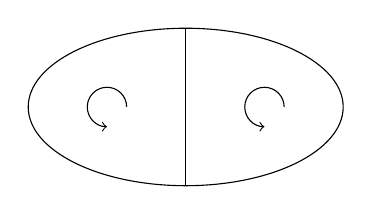
\begin{tikzpicture}
    \draw (0,0) circle[x radius=2cm, y radius=1cm];
    \draw (0,-1) -- (0,1);
    \draw [->] (-0.75,0) arc[radius=2.5mm, start angle= 0, end angle= 270];
    \draw [->] (1.25,0) arc[radius=2.5mm, start angle= 0, end angle= 270];
  \end{tikzpicture}
\end{center}

So, we define a notion of `irreducible' for \hyperlink{def:mps}{measure preserving systems}.
\begin{defi}[Ergodic]\hypertarget{def:ergodic}
  A \hyperlink{def:mps}{measure preserving system} is called \textbf{ergodic} if $A = T^{-1}A$ implies $\mu(A) = 0$ or $1$ for all $A \in \mathcal{B}$.
\end{defi}

If a \hyperlink{def:mps}{measure preserving system} is not \hyperlink{def:ergodic}{ergodic}, and we have $A \in \mathcal{B}$ with $0 < \mu(A) < 1$ such that $T^{-1} A = A$, then we can restrict the measure preserving system to $A$.
That is, we consider the measure preserving system $(A, \mathcal{B}_A, \mu_A, T|_A)$ where $\mathcal{B}_A = \set{B \in \mathcal{B} | B \subseteq A}$ and $\mu_A(B) = \frac{\mu(B)}{\mu(A)}$ for all $B \in \mathcal{B}_A$.
\begin{thm}
  The following are equivalent for an \hyperlink{def:mps}{measure preserving system} $(X, \mathcal{B}, \mu,T)$.
  \begin{enumerate}[label=(\arabic*)]
    \item $(X, \mathcal{B}, \mu, T)$ is \hyperlink{def:ergodic}{ergodic}.
    \item For all $A \in \mathcal{B}$ with $\mu(A) > 0$,
      \begin{equation*}
        \mu\left(\bigcap_{N=1}^\infty \bigcup_{n=N}^\infty T^{-n} A\right) = 1.
      \end{equation*}
    \item $\mu(A \sym T^{-1} A) = 0$ implies $\mu(A) = 0$ or $1$ $\forall A \in \mathcal{B}$.
    \item For all bounded measurable functions $f: X \to \mathbb{R}$,
      $f = f \circ T$ almost everywhere implies $f$ is constant almost everywhere.
    \item For all bounded measurable functions $f: X \to \mathbb{C}$,
      $f = f \circ T$ almost everywhere implies $f$ is constant almost everywhere.
  \end{enumerate}
\end{thm}
\begin{proof}
  (1) $\Rightarrow$ (2).
  Let $A \in \mathcal{B}$ with $\mu(A) > 0$. Let $B = \bigcap \bigcup T^{-n}A$.
  By \hyperlink{thm:poincare}{Poincar\'e recurrence}, $\mu(B) \geq \mu(A) > 0$.
  So if we show that $B = T^{-1} B$, then $\mu(B) = 1$ follows by \hyperlink{def:ergodic}{ergodicity}.
  But
  \begin{equation*}x \in B \iff x\text{ visits }A\text{ infinitely often }\iff Tx\text{ visits }A\text{ infinitely often }\iff Tx \in B.\end{equation*}
  So $B = T^{-1} B$.

  (2) $\Rightarrow$ (3). Let $A \in \mathcal{B}$ such that $\mu(A \sym T^{-1} A) = 0$. If $\mu(A) = 0$, there is nothing to prove. Suppose $\mu(A) > 0$.
  Let $B = \bigcap \bigcup T^{-n} A$. By (2), we know that $\mu(B) = 1$.

  We show $\mu(B \setminus A) = 0$, which completes the proof.
  Let $x \in B \setminus A$, then there is a first time $m$ such that $T^m x \in A$, and $m > 0$.
  Hence $x \in T^{-m} A \setminus T^{-(m-1)}A$. Thus
  \begin{equation*}
    B \setminus A \subseteq \bigcup_m T^{-m} A \setminus T^{-(m-1)} A,
  \end{equation*}
  and $\mu(T^{-m} A \setminus T^{-(m-1)} A) = \mu(T^{-1} A \setminus A) = 0$, so $\mu(B \setminus A) = 0$.

  (3) $\Rightarrow$ (4).
  Let $f : X \to \mathbb{R}$ be a bounded measurable function such that $f = f \circ T$ almost everywhere.
  For all $t \in \mathbb{R}$, let $A_t = \set{x \in X | f(x) \leq t}$.
  Then $\mu(A_t \sym T^{-1} A_t) = 0$.
  By (3), we have $\mu(A_t) = 0$ or $1$ for all $t$.

  If $t$ is very small, then $\mu(A_t) = 0$. If $t$ is very large, $\mu(A_t) = 1$. $t \mapsto \mu(A_t)$ is monotone, hence $\exists c \in \mathbb{R}$ such that $\mu(A_t) = 0$ for all $t < c$ and $\mu(A_t) = 1$ $\forall t > c$.
  Then $f(x) = c$ almost everywhere.

  (4) $\Leftrightarrow$ (5) is left as an exercise.

  (4) $\Rightarrow$ (1). Let $A \in \mathcal{B}$ with $A = T^{-1} A$. Then $\chi_A = \chi_A \circ T$ everywhere so $\chi_A$ is constant almost everywhere.
\end{proof}
\begin{eg}
  The \hyperlink{def:circ}{circle rotation} map $(\mathbb{R}/\mathbb{Z}, \mathcal{B}, \mu, R_\alpha)$ is \hyperlink{def:ergodic}{ergodic} iff $\alpha$ is irrational.
  Let $f: X \to \mathbb{R}$ be measurable. We can write $f(x) = \sum_{n \in \mathbb{Z}} a_n \exp(2\pi i n x)$.
  \begin{align*}
    f \circ R_\alpha(x) = f(x + \alpha) &= \sum_{n \in \mathbb{Z}} a_n \exp(2 \pi i n (x + \alpha)) \\
                                        &= \sum_{n \in \mathbb{Z}} a_n \exp(2\pi i n \alpha) \exp(2 \pi i n x)
  \end{align*}
  So $f = f \circ R_\alpha \iff a_n = a_n \exp(2 \pi i n \alpha) \; \forall n$. If $\alpha$ is irrational, then $\exp(2 \pi i n \alpha) \neq 1$ for all $n \neq 0$, so $a_n = 0$.
\end{eg}

% lecture 4
\clearpage
\section{Ergodic theorems}
In \marginnote{\emph{Lecture 4}}the previous section, we discussed recurrence, which is concerned with orbits visiting a particular set infinitely often.
However, we have not addressed how frequent these visits are: the second question we asked earlier.
\begin{thm}[Mean Ergodic Theorem, von Neumann]\hypertarget{thm:meanet}
  Let\hypertarget{def:invfunc} $(M, \mathcal{B}, \mu, T)$ be a \hyperlink{def:mps}{measure preserving system}, and write
  \begin{equation*}
    I \coloneqq \set{f \in L^2(X) | f \circ T = f \text{ a.e.}}
  \end{equation*}
  for the (closed) subspace of $T$-invariant functions.
  Denote by $P_T:L^2(X) \to I$ the orthogonal projection.
  Then for every $f \in L^2(X)$:
  \begin{equation*}
    \frac{1}{N} \sum_{n=0}^{N-1} f \circ T^n \to P_T f \quad \text{in } L^2(X).
  \end{equation*}
\end{thm}
\begin{thm}[Pointwise Ergodic Theorem, Birkhoff]\hypertarget{thm:pet}
  Let $(M, \mathcal{B}, \mu, T)$ be a \hyperlink{def:mps}{measure preserving system}.
  Then for every $f \in L^1(X)$, there is a $T$-invariant function
  $f^* \in L^1(X)$ such that
  \begin{equation*}
    \frac{1}{N} \sum_{n=0}^{N-1} f \circ T^n \to f^*(x) \quad \text{pointwise a.e.}
  \end{equation*}
\end{thm}

\hypertarget{def:ergavg}When $f \in L^2(X)$, then the function $f^*$ in the \hyperlink{thm:pet}{Pointwise Ergodic Theorem} is $P_Tf$.
The \hyperlink{thm:meanet}{Mean Ergodic Theorem} also holds in $L^p$ for $1 \leq p < \infty$, see the example sheet.
We call the quantity $\frac{1}{N} \sum_{n=0}^{N-1} f \circ T^n$ the \textbf{ergodic average}.

\begin{lemma}
  Let $(X, \mathcal{B}, \mu)$ be a probability space, and let $T: X \to X$ be a measurable transformation.
  Then $T$ is measure preserving if and only if
  \begin{equation*}
    \int_X f \circ T \, d\mu = \int_X f \, d\mu \label{eq:4star} \tag{$*$}
  \end{equation*}
  for all $f \in L^1(X)$.
\end{lemma}
\begin{proof}
  $(\Rightarrow)$. Let $A \in \mathcal{B}$ and note that $x \in T^{-1}(A)$ is equivalent to $Tx \in A$.
  Hence we can write
  \begin{equation*}
    \mu(T^{-1}(A))=\int\!\chi_{T^{-1}A}\,d\mu=\int\!\chi_A\circ T\,d\mu=\int\!\chi_A\,d\mu=\mu(A)
  \end{equation*}
  so $T$ is measure preserving.

  ($\Leftarrow$). As in ($\Rightarrow$), we can show \eqref{eq:4star} for characteristic functions.
  Then by linearity of integration, it also holds for simple functions.
  Now let $f \in L^1(X)$ be non-negative. Taking $f_1, f_2, \dotsc$ an increasing sequence of simple functions with $f = \lim f_n$ almost everywhere.
  Then $f \circ T = \lim f_n \circ T$ almost everywhere (since $T$ is measure preserving).
  Hence using the definition of integration and \eqref{eq:4star} for simple functions
  \begin{equation*}
    \int\!f\circ T\,d\mu=\lim\int\!f_n\circ T\,d\mu=\lim\int\!f_n\,d\mu=\int\!f\,d\mu.
  \end{equation*}
  Finally, a general $f \in L^1(X)$ can be written as the difference of two non-negative functions, and conclude \eqref{eq:4star} by linearity.
\end{proof}
\begin{defi}[Koopman operator]\hypertarget{def:koopman}
  Let $(X,\mathcal{B}, \mu, T)$ be a \hyperlink{def:mps}{measure preserving system}.
  For $f: X \to \mathbb{C}$ a measurable function, define
  \begin{equation*}
    U_T f = f \circ T
  \end{equation*}
  and call $U_T$ the \textbf{Koopman operator}.
\end{defi}
\begin{lemma}
  The \hyperlink{def:koopman}{Koopman operator $U_T$} is an isometry on the Hilbert space $L^2(X)$, i.e.
  \begin{equation*}
    \langle f, g \rangle = \langle U_T f, U_T g \rangle
  \end{equation*}
  for all $f,g \in L^2(X)$.
\end{lemma}
\begin{proof}
  Apply the previous lemma to $f \cdot \bar{g} \in L^1(X)$.
\end{proof}

\begin{defi}[Invertible]\hypertarget{def:inv}
  A \hyperlink{def:mps}{measure preserving system} $(X, \mathcal{B}, \mu, T)$ is said to be \textbf{invertible} if there is a measure preserving map $S: X \to X$ such that $T \circ S = S \circ T = \operatorname{id}_X$ almost everywhere.
  If such a map exists, denote it as $T^{-1}$.
\end{defi}
\begin{eg}
  The \hyperlink{def:circ}{circle rotation} is invertible, but the \hyperlink{def:doubling}{doubling map} is not.
\end{eg}
\begin{lemma}
  If the \hyperlink{def:mps}{measure preserving system} $(X, \mathcal{B}, \mu, T)$ is \hyperlink{def:inv}{invertible}, then \hyperlink{def:koopman}{$U_T$} is unitary on $L^2(X)$ and $U_T^* = U_{T^{-1}}$.
\end{lemma}
\begin{proof}
  We use the earlier lemma to the function $f \cdot \overline{(g \circ T^{-1})}$:
  \begin{align*}
    \langle f, \hyperlink{def:koopman}{U_{T^{-1}}} g \rangle &= \int f \cdot \overline{g \circ T^{-1}} \, d\mu \\
                                    &= \int (f \cdot \overline{(g \circ T^{-1})}) \circ T\,d\mu \\
                                    &= \int f\circ T \cdot \bar{g}\,d\mu \\
                                    &= \langle U_T f, g \rangle
  \end{align*}
  This shows that $U_T^* = U_{T^{-1}}$. Clearly $U_T U_{T^{-1}} = U_{T^{-1}} U_T = \operatorname{id}_{L^2(X)}$, so $U_T$ is unitary.
\end{proof}
The proofs we will give of the ergodic theorems rely on the idea that convergence is easy for certain special functions.

First, the ergodic averages of a $T$-invariant function $f \hyperlink{def:invfunc}{\in I}$ are equal to $f$, so they converge to $f$.
If $f = U_T g - g$ for some $g$, then the \hyperlink{def:ergavg}{ergodic averages} become telescopic sums and only the boundary terms remain, that is:
\begin{equation*}
  \frac{1}{N} \sum_{n=0}^{N-1} U_T^n(U_T g - g) = \frac{1}{N} (U_T^N g - g)
\end{equation*}
and the right hand side is easily seen to converge to $0$.
The following lemma shows that these two type of functions are enough to look at.
\begin{lemma}
  Write
  \begin{equation*}
    B \coloneqq \set{U_T g - g | g \in L^2(X)}.
  \end{equation*}
  Then $I = B^\perp$.
\end{lemma}
It is important to note that the space $B$ is not closed. So $L^2(X) = I \oplus \bar{B}$, but not every function in $L^2(X)$ is the sum of a $T$-invariant function and an element of $B$.
\begin{proof}
  We can write
  \begin{align*}
    f \in B^\perp &\iff \langle f, \hyperlink{def:koopman}{U_T} g - g \rangle = 0 \quad \forall g \in L^2(X) \\
                  &\iff \langle f, g \rangle = \langle f, U_T g \rangle = \langle U_T^* f, g \rangle \quad \forall g \in L^2(X) \\
                  &\iff f = U_T^* f.
  \end{align*}
  If the system was \hyperlink{def:inv}{invertible}, then we could finish the proof by applying $U_T = (U_T^*)^{-1}$ to both sides of the last equation.

  But, we can prove that $f = U_T f \iff f = U_T^* f$ in the general case:
  \begin{align*}
    f = U_T f &\iff \langle f - U_T f, f - U_T f \rangle = 0 \\
              &\iff\|f\|_2^2+\|U_T f\|^2_2-\langle f,U_Tf\rangle-\langle U_Tf,f\rangle=0 \\
              &\iff\|f\|_2^2+\|U_T^*\|_2^2-\langle U_T^*f,f\rangle-\langle f,U_T^*f\rangle + (\|U_Tf\|^2_2-\|U_T^*f\|_2^2) = 0 \\
              &\iff\|f-U_T^*f\|_2^2+(\|U_Tf\|_2^2-\|U_T^*f\|_2^2)=0
  \end{align*}
  Note that both terms in the left hand side of the final equation are non-negative, since $\|U_Tf\|_2=\|f\|_2$ since $U_T$ is an isometry, and $\|U_T^*f\|_2\leq\|f\|_2$ as $\|U_T^*\|=\|U_T\|=1$.

  Thus,
  \begin{equation*}
    f = U_T f \iff f = U_T^* f\text{ and }\|f\|_2 = \|U_T^*f\|_2.
  \end{equation*}
  The second statement of the right follows from the first one, hence $f = U_T f \iff f = U_T^*f$, as required.
\end{proof}
\begin{proof}[Proof of \hypertarget{thm:meanet}{Mean Ergodic Theorem}]
  Let $f \in L^2(X)$ and fix $\epsilon > 0$.
  By the lemma, we can write $f = \hyperlink{def:invfunc}{P_T} f + \hyperlink{def:koopman}{U_T} g - g + e$ for some $e, g \in L^2(X)$ such that $\|e\|_2 < \epsilon$.
  Thus
  \begin{equation*}
    \limsup_{n \to \infty} \left\|\frac{1}{N} \sum_{n=0}^{N-1} U_T^n f - P_T f\right\|_2 \leq \limsup_{n\to \infty} \left\lVert\frac{1}{N} \left(U_T^Ng - g\right) + \frac{1}{N} \sum_{n=0}^{N-1}U_T^ne\right\rVert_2 < \epsilon
  \end{equation*}
  and conclude by taking $\epsilon\to0$.
\end{proof}

\begin{thm}[Maximal ergodic theorem, Wiener]
  Let $(X, \mathcal{B}, \mu, T)$ be a \hyperlink{def:mps}{measure preserving system}.
  Let $f \in L^1$, $\alpha \in \mathbb{R}_{> 0}$. Let
  \begin{equation*}
    E_\alpha = \set{x \in X | \sup_{N > 0} \frac{1}{N} \sum_{n=0}^{N-1} f(T^n x) > \alpha}.
  \end{equation*}
  Then $\mu(E_\alpha) \leq \alpha^{-1} \|f\|_1$.
\end{thm}
\begin{prop}
  Let $(X, \mathcal{B},\mu,T)$ be a \hyperlink{def:mps}{measure preserving system}.
  Let $f \in L^1$. Let $f_0 = 0, f_1 = f, f_2 = f \circ T + f$,
  \begin{equation*}
    f_n = f \circ T^{n-1} + \dotsb + f \circ T + f,
  \end{equation*}
  and
  \begin{equation*}
    F_N = \max_{n = 0, \dotsc, N} f_n.
  \end{equation*}
  Then
  \begin{equation*}
    \int_{\set{x \in X | F_N(x) > 0}} f \, d \mu \geq 0 \; \forall N
  \end{equation*}
\end{prop}
\begin{proof}
  Suppose that $F_N(x) > 0$ for some $x$.
  Then $F_N(x) = f_n(x)$ for some $n \in \{1, \dotsc, N\}$.
  Then $F_N(x) = f_{n-1}(Tx) + f(x) \leq F_N(Tx) + f(x)$, hence
  $f(x) \geq F_N(x) - F_N(Tx)$.
  \begin{align*}
    \int_{\set{x \in X | F_N(x) > 0}} f(x)\,d\mu &\geq \int_{\set{x \in X | F_N(x) > 0}} (F_n(x) - F_N(Tx))\,d\mu \\
    \shortintertext{note if $F_n(x) \not> 0$, then $F_N(x) - F_N(Tx) \leq 0$, so}
                                                 & \geq \int_X F_N(x) - F_N(Tx)\,d\mu = 0
  \end{align*}
\end{proof}
\begin{proof}[Proof of maximal ergodic theorem]
  Define
  \begin{align*}
    E_{\alpha,M} &= \Set{x \in X | \max_{N = 1, \dotsc, M} \frac{1}{N} \sum_{n=0}^{N-1} f(T^n x) > \alpha} \\
                 &= \Set{x \in X | \max_{N = 1, \dotsc, M} \sum_{n=0}^{N-1} (f(T^n x) - \alpha) > 0}
  \end{align*}
  We apply the proposition for the function $f - \alpha$.
  Then
  \begin{equation*}
    \int_{E_{\alpha,M}} (f(x) - \alpha)\,d\mu \geq 0
  \end{equation*}
  Then
  \begin{equation*}
    \int_{E_{\alpha,M}} f(x)\,d\mu \geq \alpha \mu(E_{\alpha,M})
  \end{equation*}
  and $\int_{E_{\alpha,M}} \leq \|f\|_1$.
  Note that $E_\alpha = \bigcup_M E_{\alpha,M}$, and this is an increasing union.
\end{proof}

% let x,b,u,t be a mps. Let f in l1, then `E f* in L1, t invariant such that ...\to f*(x) pointwise ae
\begin{proof}[Proof of pointwise ergodic theorem]
  Fix $\epsilon > 0$.
  Then $\exists f_\epsilon \in L^2$, $e_{\epsilon,1} \in L^1$ such that $f = f_\epsilon + e_{\epsilon_1}$, and $\|e_{\epsilon,1}\| < \epsilon$.
  $\exists g_\epsilon \in L62$, $e_{\epsilon,2} \in L^1$ such that $f_\epsilon = P_T f_\epsilon + g_\epsilon \circ T - g_\epsilon + e_{\epsilon,2}$ and $\|e_{\epsilon,2}\|_1 < \epsilon$.

  Also, $\exists h_\epsilon \in L^\infty$, $e_{\epsilon, 3} \in L^1$ such that $g_\epsilon = h_\epsilon + e_{\epsilon,3}$ and $\|e_{\epsilon,3}\|_1 < \epsilon$.

  Thus, $f = P_T f_\epsilon + h_\epsilon \circ T - h_\epsilon + e_\epsilon$, where $e_\epsilon \in L^1$ with $\|e_\epsilon\|_1 < 4\epsilon$.

  \begin{equation*}
    \frac{1}{N} \sum_{n=0}^{N_1} f(T^nx) = P_T f_\epsilon(x) + \frac{1}{N} \left(h_\epsilon(T^N x) - h_\epsilon(x)\right) + \frac{1}{N} \sum_{n=0}^{N-1} e_\epsilon(T^nx).
  \end{equation*}
  Let
  \begin{equation*}E_{\epsilon,\alpha} = \set{x \in X | \limsup_{N \to \infty} \left|\frac{1}{N} \sum_{n=0}^\infty f(T^n x) - P_T f_\epsilon(x)\right| > \alpha}.\end{equation*}
  Applying the maximal ergodic theorem for the function $e_\epsilon$:
  \begin{equation*}
    \mu(E_{\epsilon,\alpha}) \leq \alpha^{-1} \|e_\epsilon\|_1 \leq \frac{4\epsilon}{\alpha}.
  \end{equation*}

  Let $F$ be the set of points $x$ such that $\frac{1}{N} \sum_{n=0}^{N-1} f(T^nx)$ does not converge at $x$.
  Then $F \subset \cup F_\alpha$ where
  \begin{equation*}
    F_\alpha = \set{x \in X | \limsup_{N_1, N_2 \to \infty} \left|\frac{1}{N_1} \sum_{n=0}^{N_1 - 1} f(T^n x) - \frac{1}{N_2} \sum_{n=0}^{N_2 - 1} f(T^n x)\right| > 2\alpha}.
  \end{equation*}
  Notice $F_\alpha \subset E_{\epsilon,\alpha}$ for all $\epsilon > 0$.
  $\mu(F_\alpha) \leq \mu(E_{\epsilon,\alpha}) \leq \frac{4\epsilon}{\alpha}$.
  Therefore $\mu(F_\alpha) = 0$.

  We can take a countable sequence of $\alpha$'s and conclude $\mu(F) = 0$>
  We proved that $\frac{1}{N} \sum_{n=0}^{N-1} f(T^n x) \to f^*(x)$ for some function $f^*$.

  By Fatou's lemma, $f^* \in L^1$.
  It remains to prove $f^*(x) = f^*(Tx)$ a.e.
  For a.e.\ $x$,
  \begin{align*}
    f^*(x) &= \lim_{N \to \infty} \frac{1}{N} \sum_{n=0}^{N-1} f(T^n x) \\
    f^*(Tx) &= \lim_{N \to \infty} \frac{1}{N} \sum_{n=0}^{N-1} f(T^{n+1} x) \\
     &= \lim_{N \to \infty} \frac{1}{N} \sum_{n=1}^{N} f(T^n x) \\
     &= \lim_{N \to \infty} \frac{1}{N-1} \sum_{n=1}^{N-1} f(T^n x) \\
     &= \lim_{N \to \infty} \frac{1}{N} \sum_{n=1}^{N-1} f(T^n x) \\
  \end{align*}
  Then $f^*(x) - f^*(Tx) = \lim \frac{1}{N} f(x) = 0$.
\end{proof}
\printindex
\end{document}
